\documentclass[a4paper,11pt]{article}
\usepackage{polski}
\usepackage[utf8]{inputenc}
\usepackage{enumerate}
\usepackage{mathtools}
\usepackage{amsmath}
\usepackage{graphicx} 
\author{Filip Chodorowski}
\title{Sprawozdanie z laboratorium nr 8\\
„Złożoność obliczeniowa algorytmów DFS,BFS w grafach”}
\frenchspacing
\begin{document}
\maketitle
\tableofcontents
\section{Założenia zadania}
Zadanie polegało na zaimplementowaniu struktury graf i algorytmów wyszukiwania DFS,BFS
\newpage
\section{Wyniki}
\subsection{Porównanie wyszukiwania DFS,BFS dla 10 wierzchołków przy wzroście ilości krawędzi}
\begin{center}
\begin{figure}[h!]
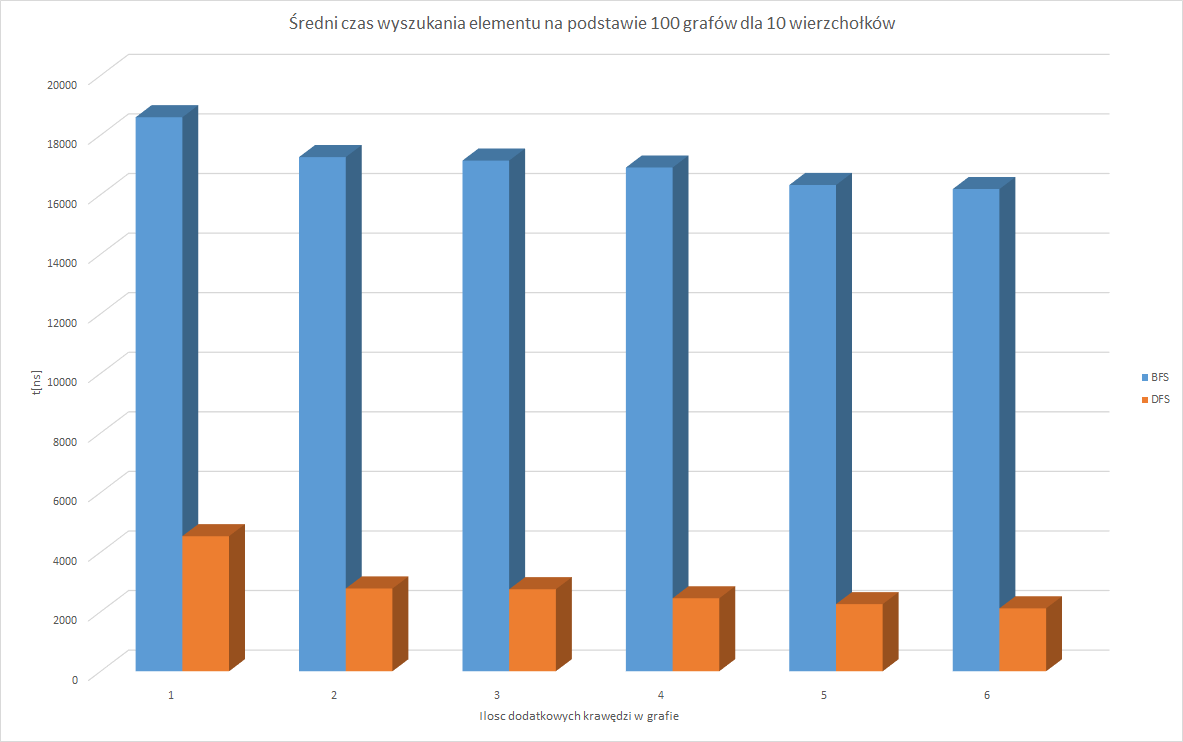
\includegraphics[width=12.5cm,height=10cm]{Wykresy2/10Wierzcholkow}
%%\caption{Tu umieszczasz opis}
\label{fig:obrazek Wykresy2/DodawanieElementow}
\end{figure}
\end{center}
Wraz ze wzrostem ilości krawędzi zmniejsza się średni czas wyszukiwania elementu. Średnia czasu wyszukiwania DFS jest krótsza niż BFS, wynika ona z mojej implementacji funkcji(więcej instrukcji do wykonania).
\newpage
\subsection{Porównanie wyszukiwania DFS, BFS dla 100 wierzchołków przy wzroście ilości krawędzi}
\begin{center}
\begin{figure}[h!]
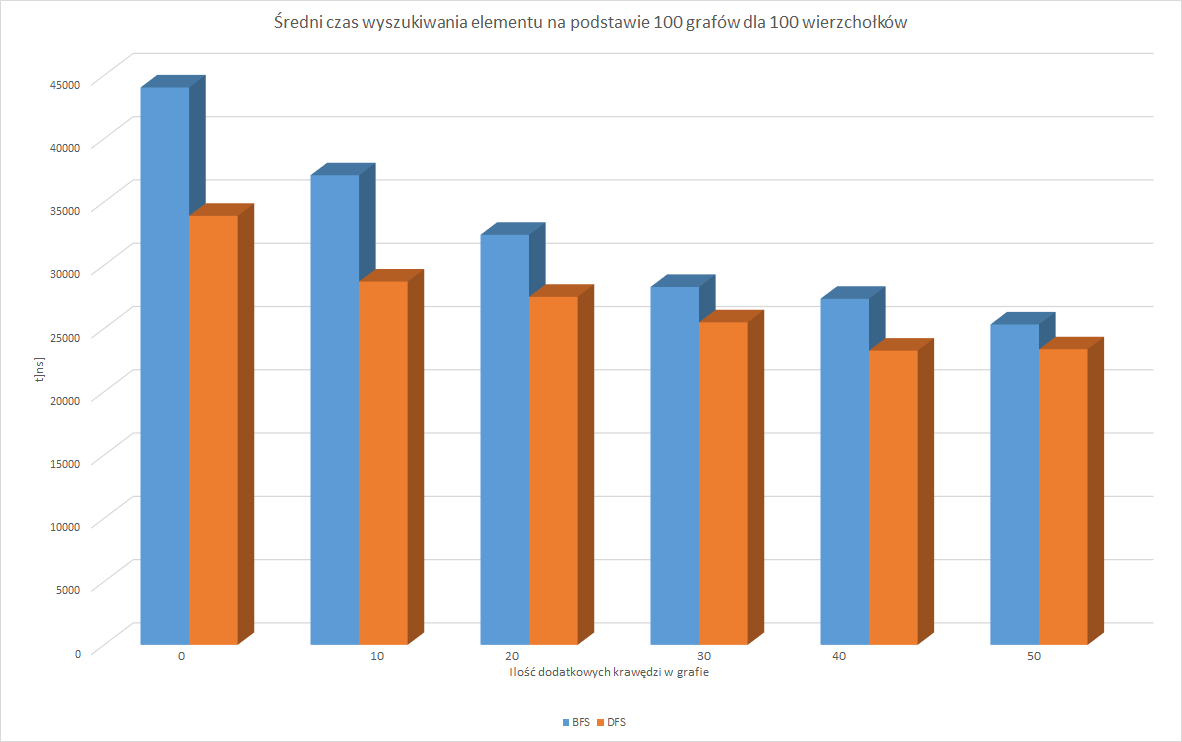
\includegraphics[width=12.5cm,height=10cm]{Wykresy2/100Wierzcholkow}
%%\caption{Tu umieszczasz opis}
\label{fig:obrazek Wykresy2/WszystkieElementyWyszukaj}
\end{figure}
\end{center}
Wraz ze wzrostem ilości krawędzi zmniejsza się średni czas wyszukania elementu.
\newpage
\subsection{Porównanie czasów wyszukiwania przy wzroście ilości wierzchołków}
\begin{center}
\begin{figure}[h!]
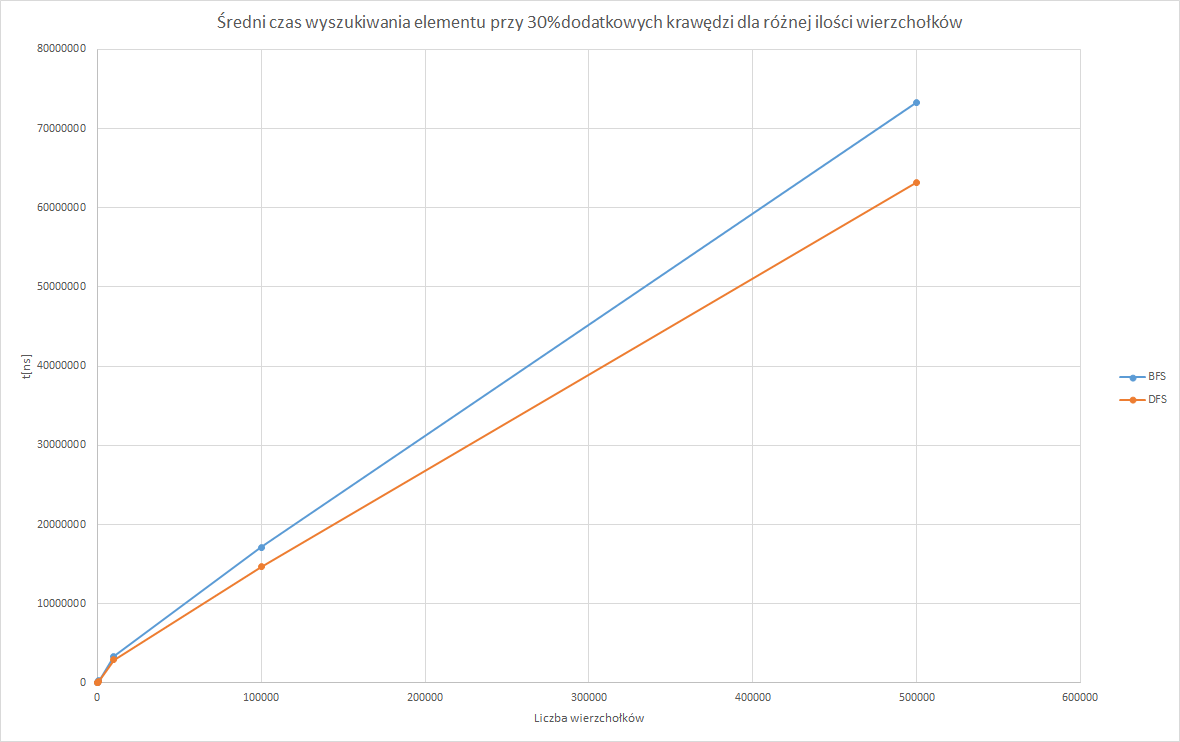
\includegraphics[width=12.5cm,height=10cm]{Wykresy2/Wykres}
%%\caption{Tu umieszczasz opis}
\end{figure}
\end{center}
Czas wyszukiwania elementu przy 30\% dodatkowych krawędzi jest tego samego rzędu dla DFS i BFS.
Złożoność wyszukiwania w grafie waha się od
$O(I)
$
do
$O(n)
$
\newpage
\subsection{Losowe wyniki}
\begin{tabular}{|r|r|r|r} \hline
BFS[ns] &DFS[ns]   &wierzcholkow &krawedzi\\    
18780& 1943&	10&				3\\
22252& 23021& 100&             30\\
49580& 165664& 1000&          300\\
81762&  26343& 1000&          300\\
16267& 3107554& 10000&       3000\\
3526334& 1391955& 10000&    3000\\ \hline
\end{tabular}
\section{Wnioski}
\begin{itemize}
%\ldots
\item Dla większego grafu szybkość znalezienia drogi zależy od umiejscowienia docelowego punktu(główny czynnik czasu działania DFS,BFS). Widać to w podrozdziale "Losowe wyniki".
\item Złożoność obliczeniowa dla obu algorytmów wynosi od 
$O(I)
$
do
$O(n)
$
\end{itemize}
\end{document}